\section{Ex2.08 Logistic map}\label{sec:LogisticMap}

\subsection{Testo esercizio}
La mappatura iterativa $$x(i+1)=rx(i)(1-x(i))$$ è chiamata \textbf{Logistic map}.

\begin{itemize}
    \item[a)] Scrivere una funzione $logisticMap(x,r)$ che ritorna il valore $x(i+1)$ 
    dati in input $x(i)$ ed $r$
    
    \item[b)] Scriver uno script con un loop per calcolare i primi $100$ passi della 
    mappa logistica partendo da $x(1)=0.5$. Memorizzare tutti i valori in una matrice $x$ 
    con $n=100$ elementi e traccia $x$ in funzione del numero di passaggi $i$.
    
    \item[c)] Esplora la mappa logistica per $$r_1=1.0\quad r_2=2.0\quad r_3=3.0\quad  
    r_4=4.0$$
    
\end{itemize}

\subsection{Svolgimento}
L'esercizio \'e stato semplice. Inizialmente avevo inserito $\rho=7500$ direttamente 
dentro la funzione, successivamente ho reputato opportuno inserire il dato via argomenti 
per rendere la funzione utile per qualsiasi tipo di sfera.

\subsection{Risultato}
\begin{figure}[h]
    \centering
    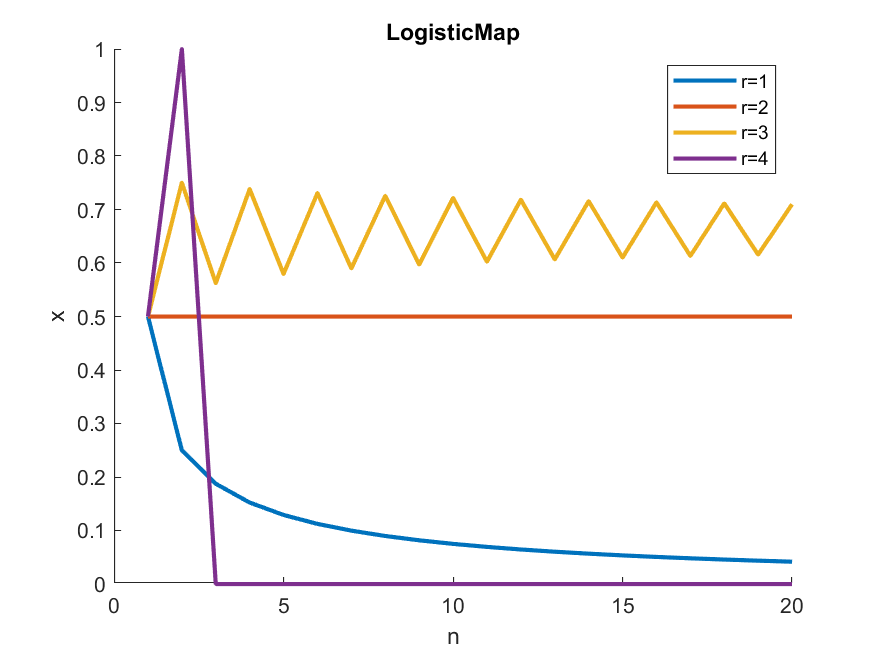
\includegraphics{cap/Elementary/img/script208}
    \GraphCap{$1/x^n$}
    \label{fig:script208}
\end{figure}

\subsection{Codice esercizio}
\lstinputlisting[caption = {\nameref{fnc:LogisticMap}},
linerange={1-3}]
{cap/Elementary/src/function/LogisticMap.m}

\lstinputlisting[title = {Script Ex2.08}]
{cap/Elementary/src/script/script208.m}
